\documentclass[11pt]{article}
% Every number and every result sentence comes from macros.tex, generated by `python -m nycemis paper`
% from results files. Do not type results into this file.
\usepackage[margin=1in]{geometry}
\usepackage{graphicx}
\usepackage{booktabs}
\usepackage{amsmath}
\usepackage[hidelinks]{hyperref}
\usepackage{natbib}
% Generated by `python -m nycemis paper`; do not edit by hand.
\newcommand{\AlphaStarML}{0.75}
\newcommand{\AlphaStarReactive}{0.75}
\newcommand{\AlphaTTBudgetPct}{5}
\newcommand{\CompositionCIHeavy}{106 to 111}
\newcommand{\CompositionCILight}{51 to 56}
\newcommand{\CompositionCIModerate}{69 to 76}
\newcommand{\CompositionHeavy}{108}
\newcommand{\CompositionLight}{54}
\newcommand{\CompositionModerate}{72}
\newcommand{\CompositionVsTTCIHeavy}{56 to 63}
\newcommand{\CompositionVsTTCILight}{56 to 61}
\newcommand{\CompositionVsTTCIModerate}{50 to 56}
\newcommand{\CompositionVsTTHeavy}{60}
\newcommand{\CompositionVsTTLight}{58}
\newcommand{\CompositionVsTTModerate}{53}
\newcommand{\CompositionWord}{mostly}
\newcommand{\ConfirmatoryN}{60}
\newcommand{\DensityHeavy}{20.75}
\newcommand{\DensityLight}{10}
\newcommand{\DensityModerate}{16}
\newcommand{\DepartDelayEcoMlHeavy}{4.0}
\newcommand{\DepartDelayEcoMlLight}{1.3}
\newcommand{\DepartDelayEcoMlModerate}{2.7}
\newcommand{\DepartDelayEcoReactiveHeavy}{2.3}
\newcommand{\DepartDelayEcoReactiveLight}{1.0}
\newcommand{\DepartDelayEcoReactiveModerate}{1.5}
\newcommand{\DepartDelayLegacyMlHeavy}{3.6}
\newcommand{\DepartDelayLegacyMlLight}{0.7}
\newcommand{\DepartDelayLegacyMlModerate}{1.5}
\newcommand{\DepartDelayRandomRerouteHeavy}{2.8}
\newcommand{\DepartDelayRandomRerouteLight}{1.1}
\newcommand{\DepartDelayRandomRerouteModerate}{1.7}
\newcommand{\DepartDelayStaticHeavy}{3.4}
\newcommand{\DepartDelayStaticLight}{0.7}
\newcommand{\DepartDelayStaticModerate}{1.7}
\newcommand{\DepartDelayTtAdaptiveHeavy}{2.1}
\newcommand{\DepartDelayTtAdaptiveLight}{1.0}
\newcommand{\DepartDelayTtAdaptiveModerate}{1.4}
\newcommand{\DetectableEffect}{2.5}
\newcommand{\DetectableMargin}{2.6}
\newcommand{\EcoCOTwoVsStaticHeavy}{-12.9}
\newcommand{\EcoCOTwoVsStaticLight}{-7.8}
\newcommand{\EcoCOTwoVsStaticModerate}{-9.2}
\newcommand{\EcoNOxVsPlaceboHeavy}{-10.0}
\newcommand{\EcoNOxVsPlaceboLight}{-10.4}
\newcommand{\EcoNOxVsPlaceboModerate}{-10.1}
\newcommand{\EcoPTTvsTTHeavy}{+6.5}
\newcommand{\EcoPTTvsTTLight}{+3.7}
\newcommand{\EcoPTTvsTTModerate}{+7.2}
\newcommand{\EcoTTvsStaticHeavy}{-10.9}
\newcommand{\EcoTTvsStaticLight}{+2.8}
\newcommand{\EcoTTvsStaticModerate}{-0.7}
\newcommand{\EcoTTvsTTHeavy}{+1.1}
\newcommand{\EcoTTvsTTLight}{+1.8}
\newcommand{\EcoTTvsTTModerate}{+2.0}
\newcommand{\EcoVkmVsStaticHeavy}{-2.2}
\newcommand{\EcoVkmVsStaticLight}{-2.4}
\newcommand{\EcoVkmVsStaticModerate}{-2.3}
\newcommand{\EdgeNOxCIHeavy}{-17.8 to -16.0}
\newcommand{\EdgeNOxCILight}{-11.0 to -10.6}
\newcommand{\EdgeNOxCIModerate}{-12.3 to -11.7}
\newcommand{\EdgeNOxHeavy}{-16.8}
\newcommand{\EdgeNOxLight}{-10.8}
\newcommand{\EdgeNOxModerate}{-12.0}
\newcommand{\EdgeNOxVsTTCIHeavy}{-8.9 to -8.5}
\newcommand{\EdgeNOxVsTTCILight}{-10.2 to -9.9}
\newcommand{\EdgeNOxVsTTCIModerate}{-9.3 to -9.0}
\newcommand{\EdgeNOxVsTTHeavy}{-8.7}
\newcommand{\EdgeNOxVsTTLight}{-10.0}
\newcommand{\EdgeNOxVsTTModerate}{-9.1}
\newcommand{\EtaStar}{1}
\newcommand{\FamilywiseAlpha}{0.05}
\newcommand{\ForecastVerdictD}{beats}
\newcommand{\ForecastVerdictR}{is worse than}
\newcommand{\ForecastVerdictV}{beats}
\newcommand{\GiniCIHeavy}{-16.9 to -16.4}
\newcommand{\GiniCILight}{-13.7 to -13.4}
\newcommand{\GiniCIModerate}{-15.0 to -14.7}
\newcommand{\GiniHeavy}{-16.6}
\newcommand{\GiniLight}{-13.5}
\newcommand{\GiniModerate}{-14.8}
\newcommand{\GiniVsTTCIHeavy}{-11.0 to -10.7}
\newcommand{\GiniVsTTCILight}{-11.8 to -11.5}
\newcommand{\GiniVsTTCIModerate}{-11.5 to -11.2}
\newcommand{\GiniVsTTHeavy}{-10.9}
\newcommand{\GiniVsTTLight}{-11.7}
\newcommand{\GiniVsTTModerate}{-11.3}
\newcommand{\HistMAER}{3.915}
\newcommand{\HistMAEV}{2.462}
\newcommand{\HorizonS}{60}
\newcommand{\HotspotPRAUCModel}{0.241}
\newcommand{\HotspotPRAUCPersistence}{0.123}
\newcommand{\JunctionBlockerS}{30}
\newcommand{\JunctionJoinM}{20}
\newcommand{\JunctionsPriority}{686}
\newcommand{\JunctionsSignal}{183}
\newcommand{\JunctionsStop}{0}
\newcommand{\LegacyBaselineHorizon}{4,132}
\newcommand{\LegacyControlledSteps}{1000}
\newcommand{\LegacyIsoRTwo}{0.30}
\newcommand{\LegacyMlHeavyChangeRate}{12.5}
\newcommand{\LegacyMlHeavyLegacyMetric}{79.8}
\newcommand{\LegacyMlHeavyMatchedMetric}{-0.61}
\newcommand{\LegacyMlLightChangeRate}{15.0}
\newcommand{\LegacyMlLightLegacyMetric}{76.4}
\newcommand{\LegacyMlLightMatchedMetric}{-0.31}
\newcommand{\LegacyMlLiteralHeavyChangeRate}{13.2}
\newcommand{\LegacyMlLiteralHeavyLegacyMetric}{79.7}
\newcommand{\LegacyMlLiteralHeavyMatchedMetric}{+0.50}
\newcommand{\LegacyMlLiteralLightChangeRate}{15.1}
\newcommand{\LegacyMlLiteralLightLegacyMetric}{76.3}
\newcommand{\LegacyMlLiteralLightMatchedMetric}{-0.09}
\newcommand{\LegacyMlLiteralModerateChangeRate}{14.5}
\newcommand{\LegacyMlLiteralModerateLegacyMetric}{76.9}
\newcommand{\LegacyMlLiteralModerateMatchedMetric}{-0.36}
\newcommand{\LegacyMlModerateChangeRate}{14.4}
\newcommand{\LegacyMlModerateLegacyMetric}{76.9}
\newcommand{\LegacyMlModerateMatchedMetric}{+0.20}
\newcommand{\LegacyNOxDropRF}{71.53}
\newcommand{\LegacyNOxDropXGB}{73.41}
\newcommand{\LegacyOldCounterRate}{13.9}
\newcommand{\LegacyRFRTwo}{0.9996}
\newcommand{\LegacyRFRunSplitRTwo}{0.9992}
\newcommand{\LegacyRecountCalls}{4,443,027}
\newcommand{\LegacyRecountChanges}{136}
\newcommand{\LegacyRecountRate}{0.003}
\newcommand{\LegacyRepeatCalls}{37,978}
\newcommand{\LegacyRepeatUnchanged}{37,978}
\newcommand{\LegacyRowRatioRF}{30.5}
\newcommand{\LegacyTestHeavyLegacyMetric}{79.1}
\newcommand{\LegacyTestHeavyMatchedChange}{+0.32}
\newcommand{\LegacyTestLightLegacyMetric}{76.6}
\newcommand{\LegacyTestLightMatchedChange}{+0.07}
\newcommand{\LegacyTestModerateLegacyMetric}{77.8}
\newcommand{\LegacyTestModerateMatchedChange}{-0.15}
\newcommand{\LegacyTestN}{60}
\newcommand{\LegacyThreshold}{2.64}
\newcommand{\ModelMAER}{3.930}
\newcommand{\ModelMAEV}{2.382}
\newcommand{\ModelRTwoR}{0.109}
\newcommand{\ModelRTwoV}{0.690}
\newcommand{\MotorwayNOxCIHeavy}{+58.0 to +65.9}
\newcommand{\MotorwayNOxCILight}{+51.4 to +61.7}
\newcommand{\MotorwayNOxCIModerate}{+56.8 to +65.0}
\newcommand{\MotorwayNOxHeavy}{+62}
\newcommand{\MotorwayNOxLight}{+56}
\newcommand{\MotorwayNOxModerate}{+61}
\newcommand{\MotorwayNOxVsTTCIHeavy}{+30.8 to +35.6}
\newcommand{\MotorwayNOxVsTTCILight}{+43.3 to +52.0}
\newcommand{\MotorwayNOxVsTTCIModerate}{+36.4 to +42.7}
\newcommand{\MotorwayNOxVsTTHeavy}{+33}
\newcommand{\MotorwayNOxVsTTLight}{+48}
\newcommand{\MotorwayNOxVsTTModerate}{+40}
\newcommand{\NPowerEq}{101}
\newcommand{\NPowerSup}{91}
\newcommand{\ObservedSDMax}{3.19}
\newcommand{\ObservedSDMin}{0.55}
\newcommand{\PCFourDirection}{Exploratory: at light demand, the 90\% CI of forecast-driven eco-rerouting (eco\_ml) vs measured-emission rerouting (eco\_reactive) (-2.99\% to -2.53\%) lies entirely below -2\%: lower NOx by more than the equivalence margin. Exploratory: at moderate demand, the 90\% CI of forecast-driven eco-rerouting (eco\_ml) vs measured-emission rerouting (eco\_reactive) (-2.52\% to -2.07\%) lies entirely below -2\%: lower NOx by more than the equivalence margin. Exploratory: at heavy demand, the 90\% CI of forecast-driven eco-rerouting (eco\_ml) vs measured-emission rerouting (eco\_reactive) (-2.36\% to -1.93\%) crosses the margin: neither equivalence nor a difference beyond the margin is shown.}
\newcommand{\PCFourHeavyCI}{-2.40 to -1.90}
\newcommand{\PCFourHeavyMean}{-2.15}
\newcommand{\PCFourHeavyPHolm}{1}
\newcommand{\PCFourHeavySentence}{At heavy demand, equivalence of forecast-driven eco-rerouting (eco\_ml) and measured-emission rerouting (eco\_reactive) within $\pm$2\% is not shown (mean -2.15\%, 90\% CI -2.36\% to -1.93\%; Holm-adjusted TOST p = 1).}
\newcommand{\PCFourLightCI}{-3.03 to -2.48}
\newcommand{\PCFourLightMean}{-2.76}
\newcommand{\PCFourLightPHolm}{1}
\newcommand{\PCFourLightSentence}{At light demand, equivalence of forecast-driven eco-rerouting (eco\_ml) and measured-emission rerouting (eco\_reactive) within $\pm$2\% is not shown (mean -2.76\%, 90\% CI -2.99\% to -2.53\%; Holm-adjusted TOST p = 1).}
\newcommand{\PCFourModerateCI}{-2.56 to -2.03}
\newcommand{\PCFourModerateMean}{-2.30}
\newcommand{\PCFourModeratePHolm}{1}
\newcommand{\PCFourModerateSentence}{At moderate demand, equivalence of forecast-driven eco-rerouting (eco\_ml) and measured-emission rerouting (eco\_reactive) within $\pm$2\% is not shown (mean -2.30\%, 90\% CI -2.52\% to -2.07\%; Holm-adjusted TOST p = 1).}
\newcommand{\PCOneHeavyCI}{-0.24 to +1.40}
\newcommand{\PCOneHeavyMean}{+0.65}
\newcommand{\PCOneHeavyPHolm}{0.00239}
\newcommand{\PCOneHeavySentence}{At heavy demand, total NOx under the legacy rule (legacy\_ml) is equivalent to no rerouting (static) within $\pm$2\% (mean +0.65\%, 90\% CI -0.09\% to +1.28\%; Holm-adjusted TOST p = 0.00239).}
\newcommand{\PCOneLightCI}{-0.06 to +0.21}
\newcommand{\PCOneLightMean}{+0.07}
\newcommand{\PCOneLightPHolm}{9.78e-11}
\newcommand{\PCOneLightSentence}{At light demand, total NOx under the legacy rule (legacy\_ml) is equivalent to no rerouting (static) within $\pm$2\% (mean +0.07\%, 90\% CI -0.04\% to +0.19\%; Holm-adjusted TOST p = 9.78e-11).}
\newcommand{\PCOneModerateCI}{-0.40 to +0.15}
\newcommand{\PCOneModerateMean}{-0.15}
\newcommand{\PCOneModeratePHolm}{1.79e-10}
\newcommand{\PCOneModerateSentence}{At moderate demand, total NOx under the legacy rule (legacy\_ml) is equivalent to no rerouting (static) within $\pm$2\% (mean -0.15\%, 90\% CI -0.36\% to +0.10\%; Holm-adjusted TOST p = 1.79e-10).}
\newcommand{\PCThreeHeavyCI}{-8.27 to -7.85}
\newcommand{\PCThreeHeavyMean}{-8.07}
\newcommand{\PCThreeHeavyPHolm}{1.79e-10}
\newcommand{\PCThreeHeavySentence}{At heavy demand, total NOx under forecast-driven eco-rerouting (eco\_ml) is lower than under travel-time rerouting (tt\_adaptive) by 8.07\% on average (95\% CI -8.27\% to -7.85\%; Holm-adjusted p = 1.79e-10).}
\newcommand{\PCThreeLightCI}{-9.43 to -9.06}
\newcommand{\PCThreeLightMean}{-9.25}
\newcommand{\PCThreeLightPHolm}{1.79e-10}
\newcommand{\PCThreeLightSentence}{At light demand, total NOx under forecast-driven eco-rerouting (eco\_ml) is lower than under travel-time rerouting (tt\_adaptive) by 9.25\% on average (95\% CI -9.43\% to -9.06\%; Holm-adjusted p = 1.79e-10).}
\newcommand{\PCThreeModerateCI}{-8.65 to -8.33}
\newcommand{\PCThreeModerateMean}{-8.49}
\newcommand{\PCThreeModeratePHolm}{1.79e-10}
\newcommand{\PCThreeModerateSentence}{At moderate demand, total NOx under forecast-driven eco-rerouting (eco\_ml) is lower than under travel-time rerouting (tt\_adaptive) by 8.49\% on average (95\% CI -8.65\% to -8.33\%; Holm-adjusted p = 1.79e-10).}
\newcommand{\PCTwoHeavyCI}{-15.67 to -14.35}
\newcommand{\PCTwoHeavyMean}{-14.95}
\newcommand{\PCTwoHeavyPHolm}{1.79e-10}
\newcommand{\PCTwoHeavySentence}{At heavy demand, total NOx under forecast-driven eco-rerouting (eco\_ml) is lower than under no rerouting (static) by 14.95\% on average (95\% CI -15.67\% to -14.35\%; Holm-adjusted p = 1.79e-10).}
\newcommand{\PCTwoLightCI}{-9.95 to -9.54}
\newcommand{\PCTwoLightMean}{-9.75}
\newcommand{\PCTwoLightPHolm}{1.79e-10}
\newcommand{\PCTwoLightSentence}{At light demand, total NOx under forecast-driven eco-rerouting (eco\_ml) is lower than under no rerouting (static) by 9.75\% on average (95\% CI -9.95\% to -9.54\%; Holm-adjusted p = 1.79e-10).}
\newcommand{\PCTwoModerateCI}{-11.32 to -10.70}
\newcommand{\PCTwoModerateMean}{-11.00}
\newcommand{\PCTwoModeratePHolm}{1.79e-10}
\newcommand{\PCTwoModerateSentence}{At moderate demand, total NOx under forecast-driven eco-rerouting (eco\_ml) is lower than under no rerouting (static) by 11.00\% on average (95\% CI -11.32\% to -10.70\%; Holm-adjusted p = 1.79e-10).}
\newcommand{\PeakDensityCIHeavy}{-37.4 to -34.1}
\newcommand{\PeakDensityCILight}{-25.5 to -24.1}
\newcommand{\PeakDensityCIModerate}{-28.4 to -27.1}
\newcommand{\PeakDensityHeavy}{-35.5}
\newcommand{\PeakDensityLight}{-24.8}
\newcommand{\PeakDensityModerate}{-27.8}
\newcommand{\PeakDensityVsTTCIHeavy}{-17.0 to -15.4}
\newcommand{\PeakDensityVsTTCILight}{-21.2 to -19.7}
\newcommand{\PeakDensityVsTTCIModerate}{-19.2 to -17.7}
\newcommand{\PeakDensityVsTTHeavy}{-16.3}
\newcommand{\PeakDensityVsTTLight}{-20.5}
\newcommand{\PeakDensityVsTTModerate}{-18.4}
\newcommand{\PersistMAER}{4.781}
\newcommand{\PersistMAEV}{3.670}
\newcommand{\PilotSD}{4.91}
\newcommand{\PlaceboNOxVsStaticHeavy}{-5.5}
\newcommand{\PlaceboNOxVsStaticLight}{+0.7}
\newcommand{\PlaceboNOxVsStaticModerate}{-1.0}
\newcommand{\PowerAtNEq}{27}
\newcommand{\PowerAtNSup}{52}
\newcommand{\PrimSecNOxCIHeavy}{-23.3 to -22.0}
\newcommand{\PrimSecNOxCILight}{-20.3 to -19.4}
\newcommand{\PrimSecNOxCIModerate}{-21.0 to -19.8}
\newcommand{\PrimSecNOxHeavy}{-23}
\newcommand{\PrimSecNOxLight}{-20}
\newcommand{\PrimSecNOxModerate}{-20}
\newcommand{\PrimSecNOxVsTTCIHeavy}{-15.8 to -14.9}
\newcommand{\PrimSecNOxVsTTCILight}{-20.6 to -19.6}
\newcommand{\PrimSecNOxVsTTCIModerate}{-17.9 to -16.9}
\newcommand{\PrimSecNOxVsTTHeavy}{-15}
\newcommand{\PrimSecNOxVsTTLight}{-20}
\newcommand{\PrimSecNOxVsTTModerate}{-17}
\newcommand{\ReactiveNOxVsStaticHeavy}{-13.1}
\newcommand{\ReactiveNOxVsStaticLight}{-7.2}
\newcommand{\ReactiveNOxVsStaticModerate}{-8.9}
\newcommand{\ReroutePeriodS}{60}
\newcommand{\ResidNOxCIHeavy}{+91.8 to +95.0}
\newcommand{\ResidNOxCILight}{+88.7 to +91.3}
\newcommand{\ResidNOxCIModerate}{+93.3 to +95.9}
\newcommand{\ResidNOxHeavy}{+94}
\newcommand{\ResidNOxLight}{+90}
\newcommand{\ResidNOxModerate}{+95}
\newcommand{\ResidNOxVsTTCIHeavy}{+64.9 to +66.6}
\newcommand{\ResidNOxVsTTCILight}{+78.2 to +80.4}
\newcommand{\ResidNOxVsTTCIModerate}{+71.8 to +74.2}
\newcommand{\ResidNOxVsTTHeavy}{+66}
\newcommand{\ResidNOxVsTTLight}{+79}
\newcommand{\ResidNOxVsTTModerate}{+73}
\newcommand{\ResidShareEcoMlHeavy}{33}
\newcommand{\ResidShareEcoMlLight}{31}
\newcommand{\ResidShareEcoMlModerate}{32}
\newcommand{\ResidSharePPCIHeavy}{+18.4 to +18.8}
\newcommand{\ResidSharePPCILight}{+16.5 to +16.9}
\newcommand{\ResidSharePPCIModerate}{+17.3 to +17.7}
\newcommand{\ResidSharePPHeavy}{+18.6}
\newcommand{\ResidSharePPLight}{+16.7}
\newcommand{\ResidSharePPModerate}{+17.5}
\newcommand{\ResidSharePPVsTTCIHeavy}{+14.6 to +14.8}
\newcommand{\ResidSharePPVsTTCILight}{+15.5 to +15.8}
\newcommand{\ResidSharePPVsTTCIModerate}{+15.0 to +15.3}
\newcommand{\ResidSharePPVsTTHeavy}{+14.7}
\newcommand{\ResidSharePPVsTTLight}{+15.6}
\newcommand{\ResidSharePPVsTTModerate}{+15.2}
\newcommand{\ResidShareStaticHeavy}{14}
\newcommand{\ResidShareStaticLight}{15}
\newcommand{\ResidShareStaticModerate}{14}
\newcommand{\ResidShareTtAdaptiveHeavy}{18}
\newcommand{\ResidShareTtAdaptiveLight}{16}
\newcommand{\ResidShareTtAdaptiveModerate}{17}
\newcommand{\ResidVehHCIHeavy}{+89.5 to +93.6}
\newcommand{\ResidVehHCILight}{+91.2 to +92.6}
\newcommand{\ResidVehHCIModerate}{+94.5 to +96.4}
\newcommand{\ResidVehHHeavy}{+92}
\newcommand{\ResidVehHLight}{+92}
\newcommand{\ResidVehHModerate}{+96}
\newcommand{\ResidVehHVsTTCIHeavy}{+66.8 to +68.0}
\newcommand{\ResidVehHVsTTCILight}{+80.3 to +81.5}
\newcommand{\ResidVehHVsTTCIModerate}{+73.7 to +75.0}
\newcommand{\ResidVehHVsTTHeavy}{+67}
\newcommand{\ResidVehHVsTTLight}{+81}
\newcommand{\ResidVehHVsTTModerate}{+74}
\newcommand{\RsrHeavy}{0.72}
\newcommand{\RsrLight}{0.95}
\newcommand{\RsrModerate}{0.85}
\newcommand{\SESOI}{2}
\newcommand{\SpeedPrimSec}{100}
\newcommand{\SpeedResid}{50}
\newcommand{\SpeedSharePrimSec}{70}
\newcommand{\SpeedShareResid}{96}
\newcommand{\SpeedShareTertiary}{96}
\newcommand{\SpeedTertiary}{80}
\newcommand{\TTNOxVsStaticHeavy}{-7.5}
\newcommand{\TTNOxVsStaticLight}{-0.6}
\newcommand{\TTNOxVsStaticModerate}{-2.7}
\newcommand{\TauAvgS}{180}
\newcommand{\TertiaryNOxCIHeavy}{-51.4 to -49.4}
\newcommand{\TertiaryNOxCILight}{-41.1 to -40.2}
\newcommand{\TertiaryNOxCIModerate}{-44.4 to -43.6}
\newcommand{\TertiaryNOxHeavy}{-50}
\newcommand{\TertiaryNOxLight}{-41}
\newcommand{\TertiaryNOxModerate}{-44}
\newcommand{\TertiaryNOxVsTTCIHeavy}{-39.5 to -38.7}
\newcommand{\TertiaryNOxVsTTCILight}{-38.0 to -37.1}
\newcommand{\TertiaryNOxVsTTCIModerate}{-38.9 to -38.0}
\newcommand{\TertiaryNOxVsTTHeavy}{-39}
\newcommand{\TertiaryNOxVsTTLight}{-38}
\newcommand{\TertiaryNOxVsTTModerate}{-38}
\newcommand{\TestHistMAED}{0.592}
\newcommand{\TestHistMAER}{3.816}
\newcommand{\TestHistMAEV}{2.426}
\newcommand{\TestModelMAED}{0.463}
\newcommand{\TestModelMAER}{3.825}
\newcommand{\TestModelMAEV}{2.347}
\newcommand{\TestPersistMAED}{0.639}
\newcommand{\TestPersistMAER}{4.611}
\newcommand{\TestPersistMAEV}{3.643}
\newcommand{\TestRuns}{360}
\newcommand{\TestSkillHistD}{+0.210 to +0.225}
\newcommand{\TestSkillHistR}{-0.003 to -0.002}
\newcommand{\TestSkillHistV}{+0.031 to +0.035}
\newcommand{\TestSkillPersistD}{+0.267 to +0.283}
\newcommand{\TestSkillPersistR}{+0.167 to +0.173}
\newcommand{\TestSkillPersistV}{+0.354 to +0.357}
\newcommand{\TestsInFamily}{12}
\newcommand{\ValidCompletionPct}{99.5}
\newcommand{\ValidTeleportPct}{0.5}
\newcommand{\VehiclesHeavy}{6,220}
\newcommand{\VehiclesLight}{2,998}
\newcommand{\VehiclesModerate}{4,797}


\title{Does forecast-driven eco-rerouting reduce simulated traffic emissions?\\
\large An audited, preregistered SUMO study of Flushing, Queens}
\author{Mohammed Y. Hossain}
\date{}

\begin{document}
\maketitle

\begin{abstract}
A 2024 student project reported that machine-learning-triggered rerouting reduced simulated NOx in Flushing,
Queens, by \LegacyNOxDropRF\% (random forest) and \LegacyNOxDropXGB\% (XGBoost). An audit of its notebook shows
that the comparison set a run of about \LegacyBaselineHorizon~s against runs stopped after
\LegacyControlledSteps~s, and that repeated rerouting calls returned unchanged routes. We rebuild the study under a
matched, preregistered protocol in SUMO: the same network, demand, fleet and seed in every condition, runs to
completion, paired seeds, a travel-time rerouting baseline and a random-rerouting placebo. Replicating the legacy
rule under this protocol, the legacy metric still reports a large drop while the matched metric does not. We then
test emission-aware rerouting driven by a \HorizonS-second traffic-state forecast against preregistered comparisons at
three demand levels; the results are stated with their confidence intervals in Section~\ref{sec:results}. All
quantities are simulated tailpipe emissions, not air quality or exposure.
\end{abstract}

\section{Introduction}
Rerouting vehicles away from congested or high-emitting streets is a natural lever for lowering urban traffic
emissions, and microscopic simulation makes such interventions cheap to test. It also makes it easy to measure
them wrongly. This paper starts from an audit of a student project whose headline result could not survive two
questions: were the compared runs the same length, and did the intervention change anything? We answer both with
the original notebook's saved outputs and with a replication, then ask the substantive question with a protocol
that removes those failure modes: does emission-aware rerouting, driven by a forecast of the next minute of
traffic, reduce network NOx compared with no rerouting, with travel-time rerouting, and with measurement-driven
eco-rerouting, and at what cost in travel time?

\section{Related work}
Route choice changes vehicle energy use and emissions, and the fastest route is not always the lowest-emission one
\citep{ahn2008route}. Eco-routing has been evaluated network-wide in simulation \citep{ahn2013ecorouting}.
Learning-based control has been studied for traffic signals with attention to air quality
\citep{fazzini2022signals,haydari2021signals} and for dynamic rerouting aimed at travel efficiency
\citep{du2021rerouting}. We use SUMO \citep{lopez2018sumo} and LightGBM \citep{ke2017lightgbm}; the statistics
use the Wilcoxon signed-rank test \citep{wilcoxon1945}, two one-sided tests for equivalence
\citep{schuirmann1987tost}, BCa bootstrap intervals \citep{efron1987bca} and Holm's procedure \citep{holm1979}.

\section{Methods}
\subsection{Scenario, demand and fleet}
The network is built from OpenStreetMap for downtown Flushing with the options of SUMO's OSM Web Wizard, clipped to
the study box, with two documented repairs (a \JunctionJoinM~m junction-join distance and SUMO's junction-blocker option at \JunctionBlockerS~s) that
remove deadlocks at one junction cluster. Demand is generated per vehicle class with the Web Wizard's trip
options and routed explicitly; three levels are calibrated on pilot seeds to a relative speed ratio (ideal over
actual travel time, relative to a near-empty network) of \RsrLight, \RsrModerate\ and \RsrHeavy\ (light,
moderate, heavy), i.e.\ \DensityLight, \DensityModerate\ and \DensityHeavy\ vehicles per hour per km of road.
Emission classes come from HBEFA~4.2 as implemented in SUMO; each vehicle's class is fixed in the route file, so all
conditions share the fleet.

\subsection{Matched protocol}
Every condition of a seed shares the network, the byte-identical route file, the SUMO seed and options; runs
continue until every vehicle has arrived. A run is valid if at least \ValidCompletionPct\% of vehicles complete and at most
\ValidTeleportPct\% teleport. The primary outcome is total NOx from SUMO's per-trip emissions.

\subsection{Controllers}
C0 keeps the free-flow routes. C1 is SUMO's travel-time rerouting device. C2--C4 set a routing weight on every
edge every \ReroutePeriodS~s, $e = (1-\alpha)\,\tau + \alpha\,\bar\tau\,m/\bar m$, where $\tau$ is the edge length over the
time-mean edge speed of the last \TauAvgS~s (floored at free-flow time, as C1's device averages its speeds) and
$m$ the per-vehicle NOx cost of traversing the edge, and reroute each vehicle every \ReroutePeriodS~s with SUMO's travel-time
router on these weights, so that at $\alpha = 0$ they reduce to travel-time rerouting. C2 (placebo) replaces the
emission term with random noise matched to C4's route-change rate ($\eta = \EtaStar$); C3 measures $m$ from the
last minute ($\alpha^* = \AlphaStarReactive$); C4 forecasts it for the next minute from traffic-state features only
($\alpha^* = \AlphaStarML$). C5 replicates the legacy rule. $\alpha^*$ was chosen on validation seeds as the value
minimising NOx with mean travel time at most \AlphaTTBudgetPct\% above C1's.

\subsection{Forecaster}
Gradient-boosted trees forecast each edge's NOx per vehicle-second and mean speed for the next minute from
sensor-like features (counts, speeds, halting, waiting, their lags and neighbours, static attributes), trained on
runs with mixed controllers and tuned on validation seeds. On validation data its mean absolute error for the
per-vehicle NOx rate is \ModelMAER\ (persistence: \PersistMAER) and for speed \ModelMAEV\ (persistence:
\PersistMAEV); hotspot PR-AUC is \HotspotPRAUCModel\ (persistence: \HotspotPRAUCPersistence).

\subsection{Statistics}
For each seed we compute the percent change of total NOx against the reference. PC2 (C4 vs C0) and PC3 (C4 vs C1)
are two-sided Wilcoxon tests; PC1 (C5 vs C0) and PC4 (C4 vs C3) are TOST equivalence tests with a margin of
$\pm$\SESOI\%. The \TestsInFamily\ tests (four comparisons times three levels) form one Holm family at \FamilywiseAlpha. The
pilot SD of paired changes (\PilotSD\%) gave $n = \ConfirmatoryN$ test seeds per condition and level, the cap of
the preregistered rule (80\% power would need $n = \NPowerSup$ for superiority and $n = \NPowerEq$ for equivalence). At
$n = \ConfirmatoryN$ the simulated power is \PowerAtNSup\% for a true change of \SESOI\% and \PowerAtNEq\% for showing
equivalence within $\pm$\SESOI\% when the true change is zero; 80\% power is reached at a true change of
\DetectableEffect\% and a margin of $\pm$\DetectableMargin\%. A non-significant test is therefore not evidence that an
effect of \SESOI\% is absent.

\section{Results}\label{sec:results}
\subsection{The legacy result}
In the legacy notebook the rerouting runs covered \LegacyRowRatioRF\% as many vehicle-steps as the baseline, and
\LegacyRepeatUnchanged\ of \LegacyRepeatCalls\ repeated reroute calls returned the unchanged route. Its predictor
is near-deterministic: $R^2 = \LegacyRFRTwo$ on a random split and \LegacyRFRunSplitRTwo\ when split by run, because
NOx is predicted from other outputs of the same emission model at the same instant. Under the matched protocol at
moderate demand, the legacy metric reports a \LegacyMlModerateLegacyMetric\% drop while the matched metric reports a
drop of \LegacyMlModerateMatchedMetric\% (a negative drop is a rise).

\subsection{Preregistered comparisons}
\PCOneLightSentence{} \PCOneModerateSentence{} \PCOneHeavySentence{}

\PCTwoLightSentence{} \PCTwoModerateSentence{} \PCTwoHeavySentence{}

\PCThreeLightSentence{} \PCThreeModerateSentence{} \PCThreeHeavySentence{}

\PCFourLightSentence{} \PCFourModerateSentence{} \PCFourHeavySentence{}

\begin{figure}[t]
\centering
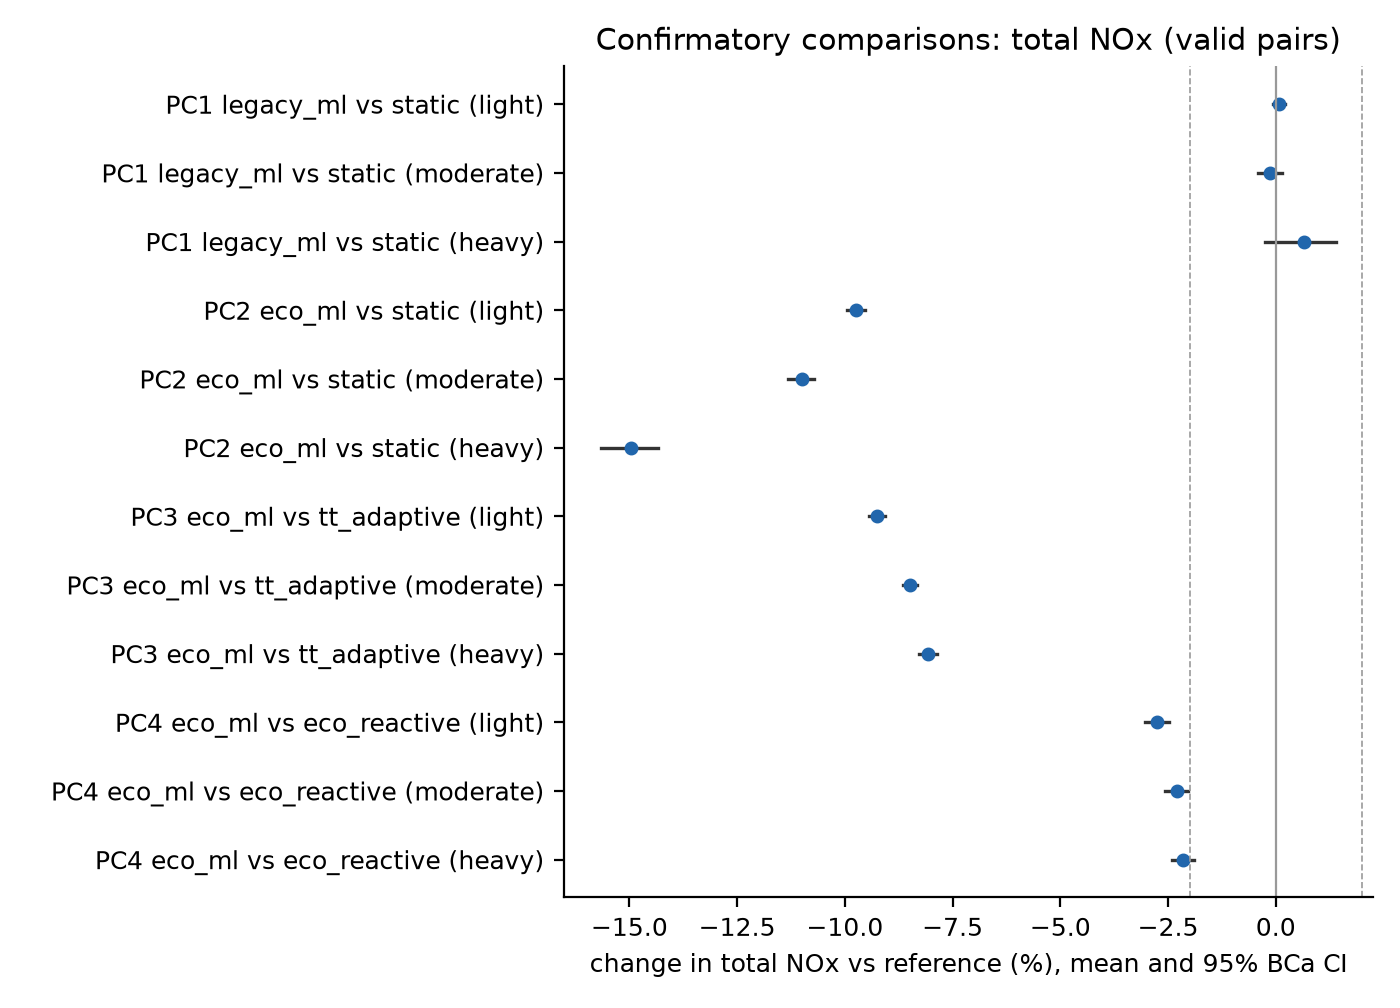
\includegraphics[width=0.9\linewidth]{figures/forest_confirmatory.png}
\caption{Preregistered comparisons: mean change in total NOx with 95\% BCa intervals; dashed lines at
$\pm$\SESOI\%.}
\end{figure}

\section{Limitations}
Demand is synthetic and not calibrated to New York counts; emission factors are European (HBEFA); there is no
dispersion, so emissions are not concentrations or exposure; the network and signals come from OpenStreetMap;
drivers comply fully; demand lasts one hour; the simulator is not validated against field measurements. No claim
here concerns health or air quality.

\section{Reproducibility}
Code, configurations, frozen inputs (with SHA-256 hashes), the preregistration and every result file are in the
repository; each stage is one command (\texttt{python -m nycemis ...}), and every number in this paper is
generated from results files.

\section*{Acknowledgments}
The original project was co-authored by Mohammed Y.\ Hossain and Billy M.\ Kyaw and supervised by Prof.\ X.\ Huang
(NYIT). Map data \copyright\ OpenStreetMap contributors, ODbL.

\bibliographystyle{plainnat}
\bibliography{refs}
\end{document}
